\documentclass[a4paper,11pt]{article}

\usepackage[utf8]{inputenc}
%\usepackage[only,llbracket,rrbracket]{stmaryrd}
\usepackage{a4wide}
\usepackage[a4paper]{geometry}
\usepackage{mathtools}
\usepackage[T1]{fontenc}
\usepackage{lmodern}
\usepackage{hyperref}
\usepackage{subcaption}
\usepackage{placeins}
%\usepackage{amssymb}
\usepackage{fixltx2e}
\usepackage{natbib}
\usepackage[crop=pdfcrop,process=auto]{pstool}
\usepackage{multirow}
\usepackage{enumerate}

\numberwithin{equation}{section}

\newcommand{\Sst}[1]{^\text{\tiny #1}}
\newcommand{\sst}[1]{_\text{\tiny #1}}

\newcommand{\diff}[2]{\frac{\mathrm{d} #1}{\mathrm{d} #2}}
\newcommand{\pdiff}[2]{\frac{\partial #1}{\partial #2}}
\newcommand{\V}[1]{\mathbf{#1}}
\newcommand{\E}[1]{\langle #1 \rangle}

\bibliographystyle{plainnat}

\title{}
\author{Matthew Russell}
\date{}

\begin{document}
\maketitle

\section{Gillespie algorithm}
The Gillespie algorithm is a stochastic simulation algorithm, named after
Gillespie due to the papers \cite{gillespie1976general,gillespie1977exact}. It
was described by Gillespie in terms of its application to simulating chemical
reactions, but it is applicable to any continuous time Markov process.
\cite{anderson2007modified} gives a clear description of the algorithm (again in
terms of chemical reactions).

\begin{figure}[ht!]
    \centering
    \psfragfig[width=0.6\textwidth]{figures/urns}
    {
        \psfrag{1}{\(1\)}
        \psfrag{2}{\(2\)}
        \psfrag{3}{\(3\)}
        \psfrag{N-1}{\(N-1\)}
        \psfrag{N}{\(N\)}
    }
    \caption{\label{fig:urns}Set up of the urns containing the particles}
\end{figure}

Suppose we have a physical system with \(N\) possible locations (``urns'') that
each particle can reside in (we impose no upper limit on the number of particles
in each urn), as in figure~\ref{fig:urns}. Denote the number of particles in urn
\(i\) by \(n_i\). Also suppose that there are \(M\)
different events that can occur in the system, such as a particle moving from
one urn to the adjacent urn, or the spontaneous appearance of a particle in the
first urn. These events must occur at specified rates, which represent the
number of times per second one expects the corresponding event to occur.  Given
the rates \(T_i, 1 \le i \le M\) at which the events in the system are expected
to occur, the basic idea of the Gillespie algorithm is to randomly choose the
time increment and then randomly choose the event that will occur at the new
time. The random time increment is drawn from an exponential distribution with
parameter \(T_0 = \sum_{i=1}^M T_i\), the sum of all of the rates. The rates of
the events are not necessarily constants and therefore must be recalculated at
each time step. For example, the rate at which a particle jumps from one urn to
an adjacent urn might depend on the number of particles in the original urn.

The Gillespie algorithm is as follows:
\begin{enumerate}[\bfseries Step 1:]
    \item Set the initial number of particles in each urn and set time \(t=0\)
    \item Calculate the rate \(T_i\) for each of the \(M\) events
    \item Set \(T_0 = \sum_{i=1}^M T_i\)
    \item Generate a uniformly random real number \(r\), such that \(0 \le r \le 1\)
    \item Set \(\delta t = \ln\left(\frac{1}{r}\right)/T_0\) (i.e. \(\delta t\)
        is drawn from an exponential distribution)
    \item Choose a event randomly from the discrete distribution such that
        probability of drawing event \(k\) is \(T_k/T_0\), for \(1 \le k \le
        M\)
    \item Increment time according to the time step, \(t \leftarrow t + \delta
        t\), and perform the changes corresponding to the event chosen
    \item Return to Step 2, unless the stopping criteria have been met
\end{enumerate}

\section{Solute transport}
Given a system as in figure~\ref{fig:urns} with \(N\) urns, we model the
transport of a solute by advection, diffusion and spontaneous disappearance of a
particle (corresponding to sinks) by the following set of events:

\begin{table}[ht!]
    \centering
    \begin{tabular}{ c | c | c | c }
        Description & Rate & Effect & Count \\ \hline\hline
        \multirow{2}{*}{Hop left} & \multirow{2}{*}{\(T^-_i = a n_{i+1}\)} &
        \(n_{i+1} \leftarrow n_{i+1} - 1\) & \multirow{2}{*}{\(N-1\)} \\
        & & \(n_i \leftarrow n_i + 1\) \\ \hline
        \multirow{2}{*}{Hop right} & \multirow{2}{*}{\(T^+_i = (a+b) n_i\)} &
        \(n_i \leftarrow n_i - 1\) & \multirow{2}{*}{\(N-1\)} \\
        & & \(n_{i+1} \leftarrow n_{i+1} + 1\) \\ \hline
        Inflow & \(T\Sst{in} = c\) & \(n_1 \leftarrow n_1 + 1\) & \(1\) \\ \hline
        Outflow & \(T\Sst{out} = d H(n_N)\) & \(n_N \leftarrow n_N - 1\) & \(1\) \\ \hline
        Removal & \(T\Sst{rem}_i = s_i H(n_i)\) & \(n_i \leftarrow n_i - 1\) & \(N\) \\
    \end{tabular}
    \caption{\label{tab:transport_events}Definitions of the different types of
events in the solute transport system}
\end{table}
Figure~\ref{fig:transport_events} gives a diagrammatic representation of the
different event types.

The constants \(a,b,c,d\) and the \(s_i\) are parameters which must be
specified, corresponding to the rates (?) of diffusion, advection, inflow,
outflow and removal (from urn \(i\)), respectively. (Maybe it only makes sense to have
\(d=a+b\)?). The rates for outflow and removal are (currently) modelling
zeroth-order kinetics and to avoid the possibility of removal when an urn is
empty, the rates involve the discrete Heaviside function, defined
here as
\begin{equation*}
    H(n) =
    \begin{dcases*}
        1 & if \(n \ge 1\)\\
        0 & if \(n < 1\)
    \end{dcases*}
\end{equation*}

There are \(M=2(N-1) + 2 + N = 3N\) events in total.
%Note that since
%the removal rate is a constant this corresponds to zero-order kinetics, where
%the removal rate does not depend on the number of particles in the urn.

\begin{figure}[ht!]
    \centering
    \begin{subfigure}[b]{0.3\textwidth}
        \centering
        \psfragfig{figures/hopleft}
        {
            \psfrag{i}{\(i\)}
            \psfrag{i+1}{\(i+1\)}
        }
        \caption{Hop left}
    \end{subfigure}
    \qquad\qquad
    \begin{subfigure}[b]{0.3\textwidth}
        \centering
        \psfragfig{figures/hopright}
        {
            \psfrag{i}{\(i\)}
            \psfrag{i+1}{\(i+1\)}
        }
        \caption{Hop right}
    \end{subfigure}

    \begin{subfigure}[b]{0.3\textwidth}
        \centering
        \psfragfig{figures/inflow}
        {
            \psfrag{1}{\(1\)}
        }
        \caption{Inflow}
    \end{subfigure}
    \qquad\qquad
    \begin{subfigure}[b]{0.3\textwidth}
        \centering
        \psfragfig{figures/outflow}
        {
            \psfrag{N}{\(N\)}
        }
        \caption{Outflow}
    \end{subfigure}

    \begin{subfigure}[b]{0.3\textwidth}
        \centering
        \psfragfig{figures/removal}
        {
            \psfrag{i}{\(i\)}
        }
        \caption{Removal}
    \end{subfigure}
    \caption{\label{fig:transport_events}Diagrammatic representation of the
different event types in the solute transport system}
\end{figure}

\FloatBarrier

\subsection{Example realisations}

\begin{figure}[ht!]
    \centering
    \psfragfig{figures/realisation1}
    {
        \psfrag{t}{\(t\)}
    }

    \caption{\label{fig:exreal1}Realisation of the time evolution of the number
of particles in each urn. \(N=10,a=1,b=0.5,c=1000,d=1.5,e=0\).}
\end{figure}

\begin{figure}[ht!]
    \centering
    \psfragfig{figures/realisation2}
    {
        \psfrag{t}{\(t\)}
    }

    \caption{\label{fig:exreal2}Realisation of the time evolution of the number
of particles in each urn. \(N=10,a=2,b=0,c=1000,d=2,e=0\).}
\end{figure}

\FloatBarrier

\section{Master equation}
The master equation describes the time evolution of the probability distribution
on the states of a continuous time Markov processes.

%Its general form is
%
%\begin{equation}
%    \label{eqn:master_eqn_general}
%    \diff{P(i,t)}{t} = \sum_j A_{ij} P(j,t),
%\end{equation}
%where \(P(i,t)\) is the probability that the system is in state with label \(i\)
%at time \(t\), and \(A_{ij}\) is a matrix of rate coefficients.

In the case of solute transport, the states of the system consist of the number
of particles contained in each urn at a given time. It is convenient to use a
vector to collect this data:
\begin{equation}
    \label{eqn:state_vector}
    \V{n} = \left(n_1,n_2, \dotsc, n_N\right)^{T}.
\end{equation}
Also, let \(T(\V{n}|\V{n}')\) denote the rate of transition from state \(\V{n}'\)
to state \(\V{n}\). Then the master equation is \citep{mckane2012stochastic}
\begin{equation}
    \label{eqn:master_eqn_rates}
    \diff{P(\V{n},t)}{t} = \sum_{\V{n}' \neq \V{n}} \left[ T(\V{n}|\V{n}')
        P(\V{n}',t) - T(\V{n}'|\V{n}) P(\V{n},t) \right].
\end{equation}

Here, \(P(\V{n},t)\) is defined as the conditional probability of finding the
system in state \(V{n}\) at time \(t\) given the initial condition that at time
\(t_0\), the system was in state \(\V{n}_0\). Or,
\begin{equation*}
    P(\V{n},t) = P(\V{n},t | \V{n}_0, t_0).
\end{equation*}

\subsection{Solute transport}
For the above problem of solute transport, the transition rates in
table~\ref{tab:transport_events} can be combined into a single object using the
notation introduced in the previous section:
\begin{equation}
    \label{eqn:}
    T(\V{n}|\V{n}') =% \left\{
        \begin{dcases*}
            a n'_{i+1} & for \(\V{n} = \V{n}' + \V{e}_i - \V{e}_{i+1},
            i=1,\dotsc,N-1\)\\
            (a+b) n'_i & for \(\V{n} = \V{n}' - \V{e}_i + \V{e}_{i+1},
            i=1,\dotsc,N-1\)\\
            c & for \(\V{n} = \V{n}' + \V{e}_1\)\\
            d H(n'_N) & for \(\V{n} = \V{n}' - \V{e}_N\)\\
            S_i H(n'_i) & for \(\V{n} = \V{n}' - \V{e}_i, i=1,\dotsc,N-1\)\\
            0 & otherwise
        \end{dcases*}
        %\right.,
\end{equation}
where \(\V{e}_i = (0,\dotsc,0,1,0,\dotsc,0)^T\) is the vector with a \(1\) in
the \(i\)-th entry and a \(0\) in all others. Using this we can write \(\V{n} =
\sum_{i=0}^{N} n_i \V{e}_i\). We will calculate the terms on the right hand side
of the master equation \eqref{eqn:master_eqn_rates} corresponding to each type
of event separately.

\begin{itemize}
    \item Hop left (\(\V{n} = \V{n}' + \V{e}_i - \V{e}_{i+1}\)):
        \begin{equation}
            \label{eqn:trans_me_hl_term}
            \sum_{i=1}^{N-1} \left[a(n_{i+1}+1) P(\V{n} - \V{e}_i +
                \V{e}_{i+1},t) - a n_{i+1} P(\V{n},t) \right]
        \end{equation}
    \item Hop right (\(\V{n} = \V{n}' - \V{e}_i + \V{e}_{i+1}\)):
        \begin{equation}
            \label{eqn:trans_me_hr_term}
            \sum_{i=1}^{N-1} \left[(a+b)(n_i+1) P(\V{n} + \V{e}_i -
                \V{e}_{i+1},t) - (a+b)n_i P(\V{n},t) \right]
        \end{equation}
    \item Inflow (\(\V{n} = \V{n}' + \V{e}_1\)):
        \begin{equation}
            \label{eqn:trans_me_in_term}
            cP(\V{n} - \V{e}_1,t) - c P(\V{n},t)
        \end{equation}
    \item Outflow (\(\V{n} = \V{n}' - \V{e}_N\)):
        \begin{equation}
            \label{eqn:trans_me_out_term}
            d H(n_N + 1) P(\V{n} + \V{e}_N,t) - d H(n_N) P(\V{n},t)
        \end{equation}
    \item Removal (\(\V{n} = \V{n}' - \V{e}_i\)):
        \begin{equation}
            \label{eqn:trans_me_rem_term}
            \sum_{i=1}^N \left[ S_i H(n_i + 1) P(\V{n} + \V{e}_i,t) - S_i H(n_i) P(\V{n},t)
                \right]
        \end{equation}
\end{itemize}

Combining \eqref{eqn:trans_me_hl_term}--\eqref{eqn:trans_me_rem_term}, we
obtain the master equation for this system:
\begin{equation}
    \label{eqn:trans_me}
    \begin{split}
        \diff{P(\V{n},t)}{t} = &
            \sum_{i=1}^{N-1} \left[a(n_{i+1}+1) P(\V{n} - \V{e}_i +
                \V{e}_{i+1},t) - a n_{i+1} P(\V{n},t) \right]\\
            +&\sum_{i=1}^{N-1} \left[(a+b)(n_i+1) P(\V{n} + \V{e}_i -
                \V{e}_{i+1},t) - (a+b)n_i P(\V{n},t) \right]\\
            +&cP(\V{n} - \V{e}_1,t) - c P(\V{n},t)\\
            +&d H(n_N + 1) P(\V{n} + \V{e}_N,t) - d H(n_N) P(\V{n},t)\\
            +&\sum_{i=1}^N \left[ S_i H(n_i + 1) P(\V{n} + \V{e}_i,t) - S_i
                H(n_i) P(\V{n},t)
                \right].
    \end{split}
\end{equation}

\section{Deterministic mean-field equations}
The objective of this section is to obtain an equation governing the time
evolution of the expected value of the number of particles in each urn.

The expected value of the entire state \(\V{n}\) at time \(t\) is
\begin{equation*}
    \E{\V{n}}(t) = \sum_{i=1}^N \langle n_i \rangle(t) \V{e}_i,
\end{equation*}
where \(\E{n_i}(t)\) is the expected value of the number of particles in urn
\(i\) at time \(t\) and is given by
\begin{align*}
    \E{n_i}(t) =& \sum_{j=0}^\infty j P(n_i = j,t)\\
    =& \sum_{j=0} j
    \sum_{\substack{\V{n} \text{ s.t.} \\ n_i=j}} P(\V{n},t)\\
    =& \sum_{j=0} j
    \sum_{n_1} \dotso \sum_{n_{i-1}} \sum_{n_{i+1}} \dotso \sum_{n_N} P(\V{n},t)\\
    =& \sum_{\V{n}} n_i P(\V{n},t),
\end{align*}
where \(P(n_i = j,t)\) denotes the marginal distribution of \(n_i\).

Differentiating \(\E{n_i}\) with respect to time,
\begin{align*}
    \diff{(\E{n_i}(t))}{t} =& \sum_{\V{n}} n_i \diff{(P(\V{n},t))}{t}.
\end{align*}

Substituting the expression \eqref{eqn:trans_me} into the above,

\begin{subequations}
\begin{align}
    \label{eqn:trans_expectation_hl_term}
    \diff{(\E{n_i}(t))}{t}
    = & \sum_\V{n} n_i \sum_{j=1}^{N-1}
    \left[a(n_{j+1}+1) P(\V{n} - \V{e}_j + \V{e}_{j+1},t) -
        an_{j+1} P(\V{n},t)\right] \\
    \label{eqn:trans_expectation_hr_term}
    + & \sum_\V{n} n_i \sum_{j=1}^{N-1}
    \left[(a+b)(n_j+1) P(\V{n} + \V{e}_j - \V{e}_{j+1},t) -
        (a+b)n_j P(\V{n},t)\right] \\
    \label{eqn:trans_expectation_in_term}
    + & \sum_\V{n} n_i
    \left[c P(\V{n} - \V{e}_1,t) - c P(\V{n},t)\right] \\
    \label{eqn:trans_expectation_out_term}
    + & \sum_\V{n} n_i
    \left[d H(n_N+1) P(\V{n} + \V{e}_N,t) - d H(n_N) P(\V{n},t)\right] \\
    \label{eqn:trans_expectation_rem_term}
    + & \sum_\V{n} n_i \sum_{j=1}^{N}
    \left[S_j H(n_j + 1) P(\V{n} + \V{e}_j,t) - S_j H(n_j) P(\V{n},t)\right]
\end{align}
\end{subequations}

We will treat the above on a term by term basis.

\paragraph{Hop left~\eqref{eqn:trans_expectation_hl_term}} We will explicitly
calculate the results for the cases \(i=1\) and \(i=N\) since the logic for
other cases is a combination of these.

\begin{itemize}
    \item \(i=1\). Evaluating the sum over \(j\) explicitly,
        \begin{align*}
            a\biggl\{
                & \sum_{n_1} \dotso \sum_{n_N} n_1 (n_2 + 1)
                P\left(\left(n_1 - 1,n_2 + 1,n_3,\dotsc,n_N\right)^T,t\right) \\
                + & \sum_{n_1} \dotso \sum_{n_N} n_1 (n_3 + 1)
                P\left(\left(n_1,n_2 - 1,n_3 +
                1,n_4,\dotsc,n_N\right)^T,t\right) \\
                + & \dotsb\\
                + & \sum_{n_1} \dotso \sum_{n_N} n_1 (n_N + 1)
                P\left(\left(n_1,\dotsc,n_{N-1} - 1,n_N + 1\right)^T,t\right) \\
                - & \sum_{n_1} \dotso \sum_{n_N} n_1 (n_2 + n_3 + \dotsb + n_N)
                P\left(\left(n_1,\dotsc,n_N\right)^T,t\right)
            \biggr\} \\
            = a\biggl\{
                & \sum_{n_1} \sum_{n_2 = 1}^\infty \sum_{n_3} \dotso \sum_{n_N} n_1 n_2
                P\left(\left(n_1 - 1,n_2,n_3,\dotsc,n_N\right)^T,t\right) \\
                + & \sum_{n_1} \sum_{n_2} \sum_{n_3=1}^\infty \sum_{n_4} \dotso
                \sum_{n_N} n_1 n_3
                P\left(\left(n_1,n_2 - 1,n_3,\dotsc,n_N\right)^T,t\right) \\
                + & \dotsb\\
                + & \sum_{n_1} \dotso \sum_{n_{N-1}} \sum_{n_N=1}^\infty n_1 n_N
                P\left(\left(n_1,\dotsc,n_{N-1} - 1,n_N\right)^T,t\right) \\
                - & \sum_{n_1} \dotso \sum_{n_N} n_1 (n_2 + n_3 + \dotsb + n_N)
                P\left(\left(n_1,\dotsc,n_N\right)^T,t\right)
            \biggr\} \\
            = a\biggl\{
                & \sum_{n_1} \dotso \sum_{n_N} \Bigl[(n_1+1)n_2 + n_1 \left(n_3
                + n_4 + \dotsb + n_N\right)\Bigr]
                P\left(\left(n_1,n_2,\dotsc,n_N\right)^T,t\right) \\
                - & \sum_{n_1} \dotso \sum_{n_N} n_1\left(n_2 + n_3 + \dotsb +
                n_N\right) P\left(\left(n_1,n_2,\dotsc,n_N\right)^T,t\right)
            \biggr\} \\
            = \hphantom{\biggl\{} a & \sum_{n_1} \dotsb \sum_{n_N} n_2
                P\left(\left(n_1,n_2,\dotsc,n_N\right)^T,t\right) \\
            = \hphantom{\biggl\{} a & \E{n_2}(t)
        \end{align*}
    \item \(i=N\). Similarly,
        \begin{align*}
            a\biggl\{
                & \sum_{n_1} \dotso \sum_{n_N} n_N (n_2 + 1)
                P\left(\left(n_1 - 1,n_2 + 1,n_3,\dotsc,n_N\right)^T,t\right) \\
                + & \sum_{n_1} \dotso \sum_{n_N} n_N (n_3 + 1)
                P\left(\left(n_1,n_2 - 1,n_3 +
                1,n_4,\dotsc,n_N\right)^T,t\right) \\
                + & \dotsb\\
                + & \sum_{n_1} \dotso \sum_{n_N} n_N (n_N + 1)
                P\left(\left(n_1,\dotsc,n_{N-1} - 1,n_N + 1\right)^T,t\right) \\
                - & \sum_{n_1} \dotso \sum_{n_N} n_N (n_2 + n_3 + \dotsb + n_N)
                P\left(\left(n_1,\dotsc,n_N\right)^T,t\right)
            \biggr\} \\
            = a\biggl\{
                & \sum_{n_1} \sum_{n_2 = 1}^\infty \sum_{n_3} \dotso \sum_{n_N} n_N n_2
                P\left(\left(n_1 - 1,n_2,n_3,\dotsc,n_N\right)^T,t\right) \\
                + & \sum_{n_1} \sum_{n_2} \sum_{n_3=1}^\infty \sum_{n_4} \dotso
                \sum_{n_N} n_N n_3
                P\left(\left(n_1,n_2 - 1,n_3,\dotsc,n_N\right)^T,t\right) \\
                + & \dotsb\\
                + & \sum_{n_1} \dotso \sum_{n_{N-1}} \sum_{n_N=1}^\infty (n_N-1) n_N
                P\left(\left(n_1,\dotsc,n_{N-1} - 1,n_N\right)^T,t\right) \\
                - & \sum_{n_1} \dotso \sum_{n_N} n_N (n_2 + n_3 + \dotsb + n_N)
                P\left(\left(n_1,\dotsc,n_N\right)^T,t\right)
            \biggr\} \\
            = a\biggl\{
                & \sum_{n_1} \dotso \sum_{n_N} n_N \left(n_2 + n_3 +
                \dotsb + n_{N-1} + (n_N - 1)\right)
                P\left(\left(n_1,n_2,\dotsc,n_N\right)^T,t\right) \\
                - & \sum_{n_1} \dotso \sum_{n_N} n_N\left(n_2 + n_3 + \dotsb +
                n_N\right) P\left(\left(n_1,n_2,\dotsc,n_N\right)^T,t\right)
            \biggr\} \\
            = - a & \sum_{n_1} \dotsb \sum_{n_N} n_N
                P\left(\left(n_1,n_2,\dotsc,n_N\right)^T,t\right) \\
            = - a & \E{n_N}(t)
        \end{align*}
    \item \(i=2,\dotsc,N-1\). For these cases we have a combination of terms of
        the type found in the cases \(i=1\) and \(i=N\):
        \begin{equation*}
            a\left(\E{n_{i+1}}-\E{n_i}\right)
        \end{equation*}
    \item The general expression for all \(i\) is
        \begin{equation*}
            \begin{dcases*}
                a\E{n_2} & for \(i=1\)\\
                a\left(\E{n_{i+1}} - \E{n_i}\right) & for \(i=2,\dotsc,N-1\)\\
                -a\E{n_N} & for \(i=N\)
            \end{dcases*}
        \end{equation*}
\end{itemize}

\paragraph{Hop right~\eqref{eqn:trans_expectation_hr_term}}
The working for the hop right terms is very similar to that for the hop left
terms above. The general expression for all \(i\):
\begin{equation*}
    \begin{dcases*}
        -(a+b)\E{n_1} & for \(i=1\)\\
        (a+b)\left(\E{n_{i-1}} - \E{n_i}\right) & for \(i=2,\dotsc,N-1\)\\
        (a+b)\E{n_N-1} & for \(i=N\)
    \end{dcases*}
\end{equation*}

\paragraph{Inflow~\eqref{eqn:trans_expectation_in_term}}
\begin{itemize}
    \item \(i=1\).
        \begin{align*}
            c \biggl\{
                & \sum_{n_1} \dotso \sum_{n_N} n_1 P\left(\left(n_1
                -1,n_2,\dotsc,n_N\right)^T,t\right) \\
                - & \sum_{n_1} \dotso \sum_{n_N} n_1 P\left(\left(n_1
                ,n_2,\dotsc,n_N\right)^T,t\right)
            \biggr\} \\
            = c \biggl\{
                & \sum_{n_1} \dotso \sum_{n_N} (n_1 + 1) P\left(\left(n_1
                ,n_2,\dotsc,n_N\right)^T,t\right) \\
                - & \sum_{n_1} \dotso \sum_{n_N} n_1 P\left(\left(n_1
                ,n_2,\dotsc,n_N\right)^T,t\right)
            \biggr\} \\
            = c \hphantom{\biggl\{} & \sum_{n_1} \dotso \sum_{n_N}
            P\left(\left(n_1,n_2,\dotsc,n_N\right)^T,t\right) \\
            = c \hphantom{\biggl\{} &
        \end{align*}
    \item \(i\ne 1\).
        All terms cancel in this case, so the result is \(0\).
\end{itemize}

\paragraph{Outflow~\eqref{eqn:trans_expectation_out_term}}
\begin{itemize}
    \item \(i=N\).
        \begin{align*}
            d \biggl\{
                & \sum_{n_1} \dotso \sum_{n_N} n_N P\left(\left(n_1
                ,\dotsc,n_{N-1},n_N+1\right)^T,t\right) \\
                - & \sum_{n_1} \dotso \sum_{n_N} n_N P\left(\left(n_1
                ,n_2,\dotsc,n_N\right)^T,t\right)
            \biggr\} \\
            = d \biggl\{
                & \sum_{n_1} \dotso \sum_{n_N} (n_N + 1) P\left(\left(n_1
                ,\dotsc,n_{N-1},n_N+1\right)^T,t\right) \\
                - & \sum_{n_1} \dotso \sum_{n_N} P\left(\left(n_1
                ,\dotsc,n_{N-1},n_N+1\right)^T,t\right) \\
                - & \sum_{n_1} \dotso \sum_{n_N} n_N P\left(\left(n_1
                ,n_2,\dotsc,n_N\right)^T,t\right)
            \biggr\} \\
            = -d \biggl\{
                & \sum_{n_1} \dotso \sum_{n_N} P\left(\left(n_1
                ,n_2,\dotsc,n_N\right)^T,t\right) \\
                - & \sum_{n_1} \dotso \sum_{n_{N-1}} P\left(\left(n_1
                ,n_2,\dotsc,n_{N-1},0\right)^T,t\right)
            \biggr\} \\
            = -d \biggl\{
                & 1 - P(n_N=0,t)
            \biggr\}
        \end{align*}
    \item \(i \ne N\).
        All terms cancel in this case due to the Heaviside function in the rates, so the result is 0.
        %\begin{align*}
        %    d \biggl\{
        %        & \sum_{n_1} \dotso \sum_{n_N} n_i P\left(\left(n_1
        %        ,\dotsc,n_{N-1},n_N+1\right)^T,t\right) \\
        %        - & \sum_{n_1} \dotso \sum_{n_N} n_i P\left(\left(n_1
        %        ,n_2,\dotsc,n_N\right)^T,t\right)
        %    \biggr\} \\
        %    = d \biggl\{
        %        & \sum_{n_1} \dotso \sum_{n_{N-1}} \sum_{n_N=1}^\infty n_i P\left(\left(n_1
        %        ,\dotsc,n_N\right)^T,t\right) \\
        %        - & \sum_{n_1} \dotso \sum_{n_N} n_i P\left(\left(n_1
        %        ,n_2,\dotsc,n_N\right)^T,t\right)
        %    \biggr\} \\
        %    = -d & \underbrace{\sum_{n_i} n_i P(n_i,n_N=0,t)}_{\text{not sure about
        %        this}}
        %\end{align*}
\end{itemize}

\paragraph{Removal~\eqref{eqn:trans_expectation_rem_term}}
\begin{align*}
    \sum_{j=1}^N S_j \biggl\{
        & \sum_{n_1} \dotso \sum_{n_N} n_i P\left(\left(n_1,\dotsc,n_{j-1},n_j +
        1,n_{j+1},\dotsc,n_N\right)^T,t\right)\\
        - & \sum_{n_1} \dotso \sum_{n_N} n_i
        P\left(\left(n_1,\dotsc,n_N\right)^T,t\right)
    \biggr\}
\end{align*}
\begin{itemize}
    \item \(i=j\) term. Similar to outflow but we now have arbitrary \(i\).
        \begin{align*}
            - S_i \biggl\{
                & \sum_{n_1} \dotso \sum_{n_N} P\left(\left(n_1
                ,n_2,\dotsc,n_N\right)^T,t\right) \\
                - & \sum_{n_1} \dotso \sum_{n_{i-1}} \sum_{n_{i+1}} \dotso
                \sum_{n_N}
                P\left(\left(n_1,n_2,\dotsc,n_{i-1},0,n_{i+1},\dotso,n_N\right)^T,t\right)
            \biggr\}\\
            = S_i \biggl\{
                & -1 + P(n_i=0,t)
            \biggr\}
        \end{align*}
    \item \(i \ne j\) terms.
        All terms cancel in the same way as the outflow case.
        %\begin{align*}
        %    & - \sum_{\substack{j=1 \\ j \ne i}}^N S_j \sum_{n_1} \dotso
        %    \sum_{n_{j-1}} \sum_{n_{j+1}} \dotso \sum_{n_N} n_i
        %    P\left(\left(n_1,\dotsc,n_{j-1},0,n_{j+1},\dotso,n_N\right)^T,t\right)
        %    \\
        %    & - \sum_{\substack{j=1 \\ j \ne i}}^N S_j \sum_{n_i} n_i
        %P\left(n_i,n_j = 0,t\right)
        %\end{align*}
\end{itemize}

\subsection{System of equations}
Let \(Y_i(t) = \E{n_i}(t), \V{Y}(t) = (Y_1(t),\dotsc,Y_N(t))^T\). Then,
collecting all the terms above and organising the system of equations in matrix
form, we obtain (neglecting the terms relating to the probability of the
number of particles in one urn to be 0).
\begin{subequations}
    \label{eqn:exp_equation_system}
    \begin{gather}
        \diff{\V{Y}}{t} = A \V{Y}(t) + \V{b},
        \intertext{where}
        A=
        \begin{pmatrix}
            -(a+b) & a & 0 & \dots & \dots & \dots & 0\\
            (a+b)  & -(2a+b) & a & 0 & \dots & \dots & 0\\
            0 & (a+b) & -(2a+b) & a & 0 & \dotsb & 0\\
            \vdots & & \ddots & \ddots & \ddots & & \vdots\\
            0 & \dots & \dots & (a+b) & -(2a+b) & a & 0\\
            0 & \dots & \dots & 0 & (a+b) & -(2a+b) & a\\
            0 & \dots & \dots & \dots & 0 & (a+b) & -a
        \end{pmatrix}
        \intertext{and}
        \V{b}=
        \begin{pmatrix}
            c-S_1\\
            -S_2\\
            \vdots\\
            -S_{N-1}\\
            -d-S_N
        \end{pmatrix}
    \end{gather}
\end{subequations}

\begin{figure}
    \centering
    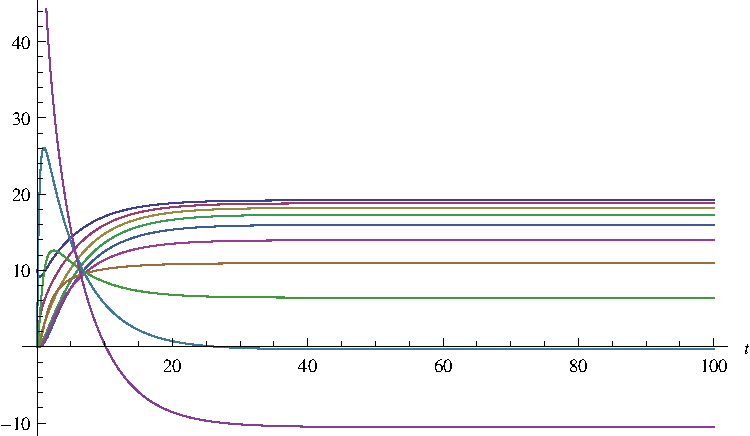
\includegraphics[width=0.8\textwidth]{figures/num_sol_exp_eq_wrong}
    \caption{\label{fig:num_sol_exp_eq_wrong}Numerical solution of
    equations~\eqref{eqn:exp_equation_system} with
\(N=10,a=1,b=0.5,c=10,d=10,S_i=0,i=1,\dotsc,N\)}
\end{figure}

\FloatBarrier
\section{Analysis of the mean-field equations}
In order to analyse the mean-field equations, we consider a 1-urn pure-death
process with death rate \(s H(n)\), where \(n\) is the number of particles in
the urn. This simple process contains many of the difficult features of the full
process above. In this case the master equation consists of the following system:

\begin{align*}
    \diff{p_0}{t} =& s p_1\\
    \diff{p_i}{t} =& s p_{i+1} - s p_i, \quad i = 2,\dotsc,N-1\\
    \diff{p_N}{t} =& - s p_N
\end{align*}
with the initial condition
\begin{equation}
    \label{eqn:pure_death_ic}
    p_i(t=0) = \delta_{iN}
\end{equation}
This means that there are surely \(N\) particles in the system at \(t=0\). We
are using the notation \(p_n(t)\) to denote the probability of there being \(n\)
particles in the urn at time \(t\).  Analogously to above, the deterministic
mean-field equation can be derived for this process:
\begin{equation*}
    \diff{\E{n}(t)}{t} = -s \left(1-p_0(t)\right).
\end{equation*}
As before, this equation is not closed. Therefore we cannot solve it exactly.
Assuming that \(p_0(t)\) is sufficiently smooth at \(t=0\), we can replace it
with its Taylor series around \(t=0\):
\begin{equation*}
    -s(1-p_0(t)) = -s\left(1 - \left[p_0(0) + \dot{p_0}(0)t +
    \frac{1}{2}\ddot{p_0}(0)t^2 + \dotsb \right] \right).
\end{equation*}

We have that \(p_0(0) = 0\) due to the initial condition. For the second term in
the series,
\begin{equation*}
    \dot{p_0}(0) = \left.(s(p_1)\right|_{t=0} = sp_1(0) = 0.
\end{equation*}
Similarly, for the next term,
\begin{align*}
    \ddot{p_0}(0) &= \left.\left(\diff{}{t}\dot{p_0}\right)\right|_{t=0}\\
    &= \left.\left(\diff{}{t}\left[s p_1\right]\right)\right|_{t=0}\\
    &= s^2\left(p_2(0) - p_1(0)\right) = 0.
\end{align*}
Continuing like this, we find that the derivatives of \(p_0(t)\) follow this
pattern:
\begin{equation*}
    p_0^{(i)}(t) = (-1)^i s^i \sum_{j=0}^{i-1}(-1)^j
    \binom{i-1}{j} p_{1+j}(t),
\end{equation*}
for \(i=1,\dotsc,N-1\).
Due to the initial condition \eqref{eqn:pure_death_ic}, we have that every
derivative is equal to \(0\) for \(i=1,\dotsc,N-1\). The expression for
\(i=N-1\) is
\begin{align*}
    p_0^{(N-1)}(t) &= (-1)^{N-1} s^{N-1} \left\{ p_1(t) - \binom{N-2}{1}p_2(t) +
    \dotsc \right.\\
    &\left.+ (-1)^{N-3} \binom{N-2}{N-3} p_{N-2}(t) +
    (-1)^{N-2}p_{N-1}(t)\right\}.
\end{align*}
Then we have
\begin{align*}
    p_0^{(N)}(t) &= (-1)^{N-1} s^{N-1} \left\{ \dot{p_1}(t) -
    \binom{N-2}{1}\dot{p_2}(t) +
    \dotsc \right.\\
    &\left.+ (-1)^{N-3} \binom{N-2}{N-3} \dot{p_{N-2}}(t) +
    (-1)^{N-2}\dot{p_{N-1}}(t)\right\}\\
    &= (-1)^{N-1} s^{N} \left\{ (p_2-p_1) -
    \binom{N-2}{1}(p_3-p_2) +
    \dotsc \right.\\
    &\left.+ (-1)^{N-3} \binom{N-2}{N-3} (p_{N-1} - p_{N-2}) +
    (-1)^{N-2} (p_N - p_{N-1})\right\}.
\end{align*}
Therefore
\begin{align*}
    p_0^{(N)}(0) &= (-1)^{N-1} (-1)^{N-2} s^N p_N\\
    &= (-1)^{2N-3} s^N
\end{align*}

Putting this together, we find that the Taylor series for \(-s(1-p_0)\) around
\(t=0\) is
\begin{align*}
    -s(1-p_0) = -s\left(1 - \left[ \frac{1}{N!}(-1)^{2N-3}s^N t^N + \dotsb
    \right] \right).
\end{align*}

From this we can see that \(p_0(t)\) grows like \(t^N\). Also, the first term is
scaled by a factor of \(\frac{s^N}{N!}\), which, for large \(N\) is very small.

\section{Todo/problems}
\begin{itemize}
    \item Get to the bottom of the non-closed system for the mean-field
        \begin{itemize}
            \item The problem is caused by the ``nonlinear'' transition rates
                (i.e. not a linear function of \(n\)) which gives us an
                absorbing boundary at \(n=0\)
            \item Looked at generating functions, ``limbo states'' etc. and
                these don't seem to solve the problem in this case
            \item Might be more feasible to use a continuous description
                (something like Fokker-Planck)
        \end{itemize}
    \item Read about Fokker-Planck equations and related
    \item Try to derive continuous version of the multiple urns problem
\end{itemize}


\bibliography{references}

\end{document}
